\section{Formal Foundations - Logic of Events}
\label{sec_logic}

This chapter introduces the logical and programmatic foundations needed for this
thesis. To achive this, it is split into two parts. The first part introduces
the reader to the Logic of Events which is the theoretical foundation for the
Velisarios framework. The second part provides a practical introduction to
the basics of COQ and programming with Velisarios.

\subsection{Logic}

The Logic of Events was introduced by Bickford and
Constable~\cite{bickford2003logic} to describe parallel systems which
consists of nodes and events happening between them. To follow
the explanation a brief overview about propositional logic, predicativ logic,
constructive logic and type theorie is presented. It is assumed that the reader
is already familiar with the basic logical systems.

\paragraph{Propositional Logic}
The oldest known logic uses atoms or a set of primitive symbols and logical
connective or a set of operator symbols to formalize
terms or propositions about the world. Statements in classical logic can be either
\textbf{true} or \textbf{false}. The table~\ref{tab:proplogic} provides
a short description for the logical connectives and their meaning.~\cite{heinemann2013logik}

\begin{table}[h]
  \centering
  \begin{tabular}{c|c|l}
    Symbols & Example & Description\\\hline
    $A,B,C,...$ & $P, Q$ & Atoms used in propositions.\\
    $\neg$ & $\neg P$ & Negation of some atom or proposition.\\
    $\vee$ & $P \vee Q$ & The disjuction of two propositions.\\
    $\wedge$ & $P \wedge Q$ & The conjunction of two propositions.\\
    $\Rightarrow$ & $P \Rightarrow Q$ & The implication of two propositions.\\
    $\Leftrightarrow$ & $P \Leftrightarrow Q$ & The equivalence composed of two propositions.\\
  \end{tabular}
  \caption{Overview of propositional logic symbols}
  \label{tab:proplogic}
\end{table}

To make sense out these defined terms these need to be evaluated. To do so,
the atoms are assigned to thruth values which is called the \textit{interpretation}.~\cite{tuschik1994mathematische}

\begin{defi}
  More formal, an interpreation is a sample assigned for a term $t$ with
  $I:L(t)\rightarrow \{true,false\} \leftrightarrow t^I$. Interpretation which satisfies the term
  $t^I$ are called a \textit{model}.
\end{defi}

Most defined formal systems are using terms which are taken as truth without
proof or justification. These terms are called \textit{axioms}. These are syntactically
without meaning but semantically always true.~\cite{tuschik1994mathematische}

To gather new knowledge out of axioms, terms and atoms a way to conclude
new terms is needed. This can be done by adding \textit{inference rules} to
the system. These rules derive new terms oder conclusions out of a given
set of propositions. Such a formal system is called \textit{logical calculus}.~\cite{tuschik1994mathematische}

\paragraph{Predicate Logic}
The predicate logic is an extension of the propositional logic.
For instance, the statement ``x is a prime number'' can't be described
in propositional logic since the thruth value depends on the structure of $x$.
The predicate logic adds \textit{quantifiers} and \textit{predicates} to the
system to describe atoms with variable structures.~\cite{heinemann2013logik}

\begin{table}[h]
  \centering
  \begin{tabular}{c|c|l}
    Symbols & Example & Description\\\hline
    $a,b,...$ & $x,y$ & The set of variables $\mathcal{V}$.\\
    $P_0^n,Q_1^n,...$ & $P(x_1,...,x_n)$ & The set of predicates $\mathcal{P}$ with arity $n$\\
            & &                           which evaluates to $\{true,false\}$\\
    $f_0^n,g_1^n,...$ & $f(t_1,...,t_2)$ & The set of formulas $\mathcal{F}$with arity $n$\\
    $\forall$ & $\forall x.P(f(x))$ & The quantifier means that for all possible\\
            & & allocations the term holds.\\
    $\exists$ & $\exists x.P(x)\Rightarrow Q$ & The quantifier means that for some\\
    & & allocations the term holds.\\
    $=$ & $x = y$ & The equality is added as connective to the alphabet.\\
  \end{tabular}
  \caption{Overview of predicate logic symbols}
  \label{tab:predlogic}
\end{table}

The table\,\ref{tab:predlogic} presents the extension made by the predicate logic.
Since the predicate logic is mathematically used to describe objects,
structure and their relations it is useful to define such structures.~\cite{heinemann2013logik}

\begin{defi}
  The type $T$ is a pair of $(I,J)$ where $I\subseteq P$ and $J\subseteq F$.
  Therefore, predicates are relations between objects of the underlying
  structure.
\end{defi}

The interpretation is similar to propositional logic execept it is
extended with $n$-artity predicate- and function symbols.~\cite{heinemann2013logik}

\paragraph{Intuitionistic Logic}
The propositional and predicate logic are presented with the classical
interpretation. The classical interpretation assumes that every statement
is either $true$ or $false$ or more elaborated a mathematical object either
exists or not. Therfore, proofs with classical interpretation don't care
about how such an object is constructed. For example the law of double
negation eliminitation  $\neg\neg A\Rightarrow A$ or the Aristotelian law of excluded
middle $A \vee \neg A$, are such problematic laws. These laws don't provide
intrinsic justification, in the way that they don't construct an object
of that type or prove that it ``exists''.~\cite{sep-logic-intuitionistic, kreitz1994automatisierte}

This problem was found by Brouwer in 1908. He observed that $A \vee \neg A$
applied on infinite sets lead to problems. An example is the Goldbach
conjecture which assumes that every number $> 2$ can be expressed as the
sum of two prime numbers. The classical logic uses a wider interpretation
the law of excluded middle to get around this problem. It assumes
that one of the cases must be true and none of them is not an option.
As a side-effect such an interpretation rejects to be generally
applicable to mathematical computational models.~\cite{sep-logic-intuitionistic, sep-mathematics-constructive}

The \textit{intuitionism} is a mathematical direction of thinking which
rejects the line of argument and universality of the law of excluded middle
and other laws of that type. For this reason, the intuitionism demands
that mathematical statements are seen as constructive statements.
For instance, the exists quantifier $\exists x.A$ is re-interpreted in a way
that a real object can be given and is not only a theoretical one.
Logical connective are also re-interpreted that they give a way
of constructing a proof with real objects and at every time one can
know which way the proof uses. One can see from the \textit{evidence}
of some proof with the disjunction $A\vee B$ which part of the disjunction
leads to a correct proof.~\cite{kreitz1994automatisierte}

\begin{table}[h]
  \centering
  \begin{tabular}{c|l}
    Symbols &  Description\\\hline
    $q$ & Every literal $q$ has some evidence $e$.\\
    $P\vee Q$ & The proof demands either an evidence for $P$ or $Q$ and mark it.\\
    $P\wedge Q$ & The proof demands an evidence for both $P$ and $Q$.\\
    $P\Rightarrow Q$ & The proof demands an effective algorithm which\\
           & converts every proof for $P$ into one for $Q$.\\
    $\neg P$ & To proof the abscence one must show that there is no proof for it.\\
    $\exists x:T.P(x)$ & The proof needs a constructed object of type $T$ which holds for $P$.\\
    $\forall x:T.P(x)$ & The proofs demands that for every object $x$ out of the type $T$\\
                 &  $P$ there is an effective algorithm which computes a proof.
  \end{tabular}
  \caption{Intuitionistic interpretation of the typed predicate logic~\cite{sep-mathematics-constructive}}
  \label{tab:intsymbols}
\end{table}

Table~\ref{tab:intsymbols} shows the intuitionistic interpretation for the logical
symbols in typed predicate logic. As an application example, proofs about
programs can only be done \textit{constructivly} since a proof of contradiction
says nothing about how to construct such a program or if the program
fulfills some property.~\cite{kreitz1994automatisierte}
Therefore, within the rest of this theses logical
statements uses the intuitionistic logical interpretation.

\paragraph{proofs-as-programs}
Taken the intuitionistic interpretation into computer science then for
mathematical questions the result is a piece of code which can be
executed. This means, that for some typed piece of code the same
rules apply as well as for the intuitionistic logic. They're
fundamentally the same concept in different areas.
For instance, an elementary programming problem consists of
some specification or formula in a logical theory and as a solution
some computational function satisfying the formula. At least, the
proof is the explanation or link between the specification and the
solution.~\cite{bates1985proofs}
This paradigm is called \textit{proofs-as-programs} and the foundation
for modern theoretical work where programs are written by proofing their
specification with the help of some theorem prover. The extracted executable
functional program is called a~\textit{realizer} for the proof.

\begin{table}[h]
  \centering
  \begin{tabular}{c|c}
    Type & Proposition\\\hline
    Type variable $a'$ & Atomic proposition $A$\\
    Function type $\rightarrow$ & Implication $\Rightarrow$\\
    Product type $*$ & Conjunction $\wedge$\\
    Union type $+$ & Disjunction $\vee$\\
    \texttt{unit} & \textit{true} \\
    \texttt{void} or type without values & \textit{false}\\
    $A\rightarrow \{\}$ & Negation $\neg$ \\
  \end{tabular}
  \caption{The isomorphism between types and logic.}
  \label{tab:proofsasprogs}
\end{table}

Table~\ref{tab:proofsasprogs} shows the Curry-Howard isomorphism between
logical proposition and types used to describe function behavior.

As an example consider the statement
\[
  \forall x:T.\exists y:S.R(x,y)
\]
which can be transformed into a program $f$ from the type $T\rightarrow S$.
The function $f$ holds for any $x\in T$ with $R(x,f(x))$ is true.
Modern theorem proving systems extract the constructive content and
produce the function described by the proof automatically.
The resulting function is \textit{extracted} from the proof
and can be simulated or run on a real system.~\cite{bickford2009component}
Such functions are also called \textit{correct-by-construction}.

Over the last decades new constructive methods are developed which
extend the proofs-as-programs paradigm by applying it to distributed
systems. Such programs are not pure functional which means they have
side-effects, an internal state, multiple agents in a system which
communicate via messages and so forth. Extracting programs
are much harder since the specification is inherently tied to
the logical structure of distributed systems. These logical
structures are called \textit{event structures} and one of these
is the \textit{logic of events}.~\cite{bickford2009component}


\subsection{Logic of Events}
The following section presents the logical language \textit{logic of events},
presented by Mark Bickford and Richard L. Constable in different
papers~\cite{bickford2003logic, bickford2005causal, bickford2009component}.

The logic of events is an approach to find an adequate logic for distributed
systems. It should bear the power of explaining and providing the
technical needs for a constructive logic. The logic builds on an
abstract high level without the binding to a specific computational
oder executional model. This provides room for the creative building
of distributed systems and their verification. Therefore, the realization
is excluded because it needs a deep understanding of systems programming.
These can be implemented and verified on another level an provided for
the logic of events as realizer or extractor.~\cite{bickford2005causal}

The main idea is to describe a causal system which is defined by it's
behavior on cause and effect, like in interacting computational systems
or likewise physical systems.~\cite{bickford2005causal}
The ideas are based on the early work from Lamport on ``Time, clocks, and
the ordering of events in a distributed system''~\cite{lamport1978time}
and Winskel on ``An introduction to event
structures''~\cite{winskel1988introduction}.

The atomic building blocks of the theory are events. These are action
in space and time which are considered to be instantaneous.

\begin{defi}
  Two events $e$ and $e'$ are causally ordered which is denoted by $e<e'$.
\end{defi}

The event structure is determined by events happening at discrete and separate
points which are called \textit{entities} or \textit{loci}. Actions or events
are located at these locus and the set of loci can change over time.
Each loci can have different properties which are identified by some
\textit{key} and have some type $T$. These are properties are
\textit{observables} and their value can be measured somehow.
The list of observables at some locus is called its \textit{state}.
The interaction which happens between the entities relays on
\textit{communication channels} which allows the entities to send
\textit{messages} (actions) to each other. The channel structure
can be dynamic but the links are relaible and messages can't be blocked.
Two types of messages are distinguished. The first one is an
external one which is recieved by another entity and the other on is triggered
by the entity itself in response to a former event.~\cite{bickford2005causal}

\begin{figure}[ht]
  \centering
  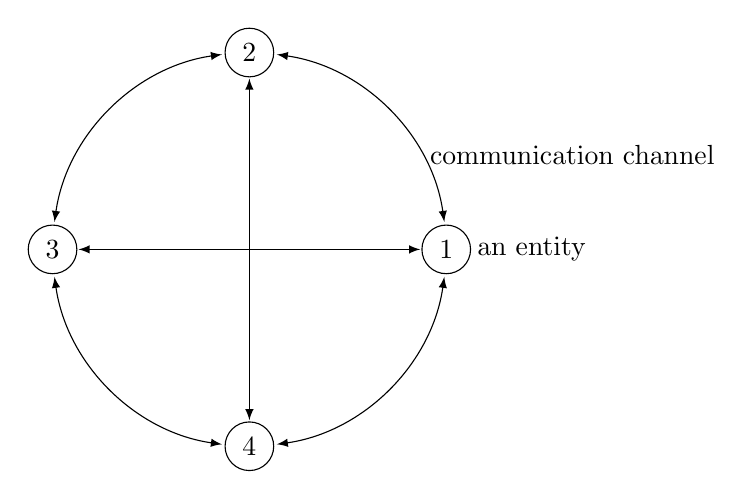
\begin{tikzpicture}

    \def \n {4}
    \def \radius {2.5cm}
    \def \margin {8} % margin in angles, depends on the radius
    % define coordinates for nodes
    \coordinate (A) at ({360/\n * (1 - 1)}:{\radius-3.3mm});
    \coordinate (B) at ({360/\n * (2 - 1)}:{\radius-3.3mm});
    \coordinate (C) at ({360/\n * (3 - 1)}:{\radius-3.3mm});
    \coordinate (D) at ({360/\n * (4 - 1)}:{\radius-3.3mm});
    %\coordinate (E) at ({360/\n * (5 - 1)}:{\radius-3.3mm});
    
    % draw the circle
    \foreach \s in {1,...,\n}
    {
      \node[draw, circle] (\n) at ({360/\n * (\s - 1)}:\radius) {$\s$};
      \draw[<->, >=latex] ({360/\n * (\s - 1)+\margin}:\radius) 
      arc ({360/\n * (\s - 1)+\margin}:{360/\n * (\s)-\margin}:\radius);
    }
    % draw the mesh and labels
    \draw[<->, >=latex] (A) -- (C);
    % \draw[<->, >=latex] (A) -- (D);
    \draw[<->, >=latex] (B) -- (D);
    % \draw[<->, >=latex] (B) -- (E);
    % \draw[<->, >=latex] (C) -- (E);
    \node at (A) [right=+6mm] {an entity};
    \node at (A) [above=+12mm,right] {communication channel};
  \end{tikzpicture}
  \caption{A possible event structure}
  \label{fig:structure}
\end{figure}

Figure~\ref{fig:structure} shows an example network of five nodes which
are all linked together. Each of the four nodes ($A..D$) can have some internal
and maybe observable state and messages are send over the communication channels
to the other entities of the network. 

The underlying computational model for the entities or nodes is the
message automata. This follows the assumption that ``the universe is run by
computation''~\cite{bickford2005causal} and everything can be modelled
by functionally updating the state and the message queues on the communication
channels of some entity. The proposed update function is $s':=f(s,v)$ where
the next state $s'$ follows from the current state $s$ and some internal or
external message $v$. $f$ is some arbitrary function which computes
the update step.~\cite{bickford2005causal}

To axiomatize these structure two types which are disjoint and two partial
functions are needed. The equality of the types are decidable.

\begin{defi}
  The large type of discrete types is
  $\mathcal{D}:=\{T:Type\ |\ \forall x,y:T.x=y\ in\ T\vee\neg (x=y\ in\ T)\}$.
  \textnormal{~\cite{bickford2005causal}}
\end{defi}

\begin{table}[h]
  \centering
  \begin{tabular}{l|l}
    Elements & Description\\\hline
    \textbf{E}$:\mathcal{D}$ & The type of possible discrete events.\\
    \textbf{Loc}$:\mathcal{D}$ & The type of possible discrete entities.\\
    \textbf{pred?}$:E\rightarrow (E+Loc)$
             & Return either the preceding event of\\
             & a location or the location itself.\\
    \textbf{sender?}$:E\rightarrow (E+Unit)$
             & Return the event which sents $e$ if e was sent or nothing.\\
  \end{tabular}
  \caption{The main types and functions for ordered event structures.~\cite{bickford2005causal}}
  \label{tab:eorder}
\end{table}

Table~\ref{tab:eorder} shows the signature of event structures with order.

From these functions we derive the next ones using the $is\_left$ which decides
on union types $(A+B)$ if the element is on the left side.
The function \[first(e)=\ if\ is\_left(pred?(e))\ then\ true\ else\ false\]
returns true if $e$ is the first event happening at some location.
The other function derived is $recv?(e)=\ if\ is\_left(sender?(e))\ then\ true\
else\ false$ returns true if the event $e$ was sent by another event.~\cite{bickford2005causal}

From these function we define the order relation.

\begin{defi}
  The strongly well-founded oder relation is
  $pred!(e,e') == (\neg first(e') \Rightarrow e = pred?(e')) \vee e = sender(e')$.
  This is the causal order relation from Lampert and denoted by $e<e'$.
\end{defi}

Additionally, there are three axioms that are needed to constraint the
event structure.~\cite{bickford2005causal}

\begin{axiom}
  If there is an event $e$ which triggers another event, then there is an
  event $e'$ such that for any event $e''$ which got triggered, $e''=e'$
  or $e''<e'$.
  \[\forall e:E.\exists e':E.\forall e'':E.(recv?(e'')\&sender?(e'')=e)\Rightarrow (e''=e'\vee e''<e)\]
\end{axiom}

\begin{axiom}
  The function $pred?$ is injective.
  \[\forall e,e':E.loc(e) = loc(e')\Rightarrow pred?(e) = pred?(e')\Rightarrow e=e'\]
\end{axiom}

\begin{axiom}
  The function $pred!$ is strongly well founded.
  \[\exists f:E\rightarrow \mathbb{N}.\forall e,e':E.pred!(e,e')\Rightarrow f(e)<f(e')\]
\end{axiom}

Axiom 3 can be explained as a ``tour'' through the event structure where
events happen as they're examined on the tour. This means that local
events are linearly ordered at each location and a recieve only happens
after a corresponding send.~\cite{bickford2005causal}

From that assumptions we define the finite list of events before a given event as
\[before(e):=\ if\ first(e)\ then\ [\,]\ else\ pred?(e)\ append\ before((pred?(e)))\] 
and likewise the finite tree of all events causally before e as
\begin{align*}
  prior(e):= & if\ first(e)\ then\ [\,]\ else\\
             & if\ recv?(e)\ then\ <e,prior(sender?(e)),prior(pred?(e))>\\
             & else\ <e,prior(pred?(e))>
\end{align*}

This basic language allows to describe event structures but to make
it more useful events should send values to each other. To distinguish
between internal events a discrete type called Act is used.~\cite{bickford2005causal}

\begin{defi}
  The type of an event is $kind :=\ Act + Top$ where $Act$ is some
  internal action and right some external one. The corresponding function
  $kind: E\rightarrow Act + Top$ returns the value of some event.
\end{defi}

\begin{defi}
  $Ty:Loc\rightarrow kinde\rightarrow Type$ returns the type of some event value at some specific
  node. For internal events $val:E\rightarrow Ty(loc(e),kind(e))$ can be any element of
  $Ty(e,a)$ choosen by any method.
\end{defi}

\begin{figure}
  \center
  \begin{tikzpicture}[node distance=2cm,auto,>=stealth]
    \node[] (server) {$B$};
    \node[left = of server] (client) {$A$};
    \node[below of=server, node distance=3cm] (server_ground) {};
    \node[below of=client, node distance=3cm] (client_ground) {};
    % vertical line
    \draw (client) -- (client_ground);
    \draw (server) -- (server_ground);
    % horizontal lines
    \draw[->] ($(client)!0.2!(client_ground)$) node[above,scale=0.5,left]{$a_1(3)$} -- ($(server)!0.3!(server_ground)$) node[above,scale=0.5,right] {$recv(3)$};
    \draw[<-] ($(client)!0.5!(client_ground)$) node[above,scale=0.5,left]{$recv(4)$} -- ($(server)!0.4!(server_ground)$) node[above,scale=0.5,right]{$b_1(4)$};
    \draw[->] ($(client)!0.6!(client_ground)$) node[below,scale=0.5,left]{$a_2(5)$} -- ($(server)!0.7!(server_ground)$) node[below,scale=0.5,right]{$recv(5)$};
    \draw[<-] ($(client)!0.9!(client_ground)$) node[below,scale=0.5,left]{$recv(6)$} -- ($(server)!0.8!(server_ground)$) node[below,scale=0.5,right]{$b_2(6)$};
  \end{tikzpicture}
  \label{fig:sequence}
  \caption{A message sequence diagram with an event structure between to
    processes A and B.}
\end{figure}

Figure~\ref{fig:sequence} shows a simple event structure between two
processes. The process $A$ sends a natural number to process $B$ which adds
one to the value and retuns the result.

To model the fact that an event $e$ can depend on a previous event $e'$ at
some location the notion of state and three relations are introduced.~\cite{bickford2005causal}

\begin{defi}
  $Identifiers$ $Id:\mathbb{D}$ are the discrete type of names of state variables where each
  holds a value with some specific type $T:x:Id\rightarrow i:Loc\rightarrow Type$.
\end{defi}

\begin{defi}
  For each location $i$ the state is the mapping of $Id\rightarrow T(x,i)$.
  The relations are \textbf{initially:} $x:Id\rightarrow i:Loc\rightarrow T(x,i)$,
  \textbf{when:} $x:Id\rightarrow e:E\rightarrow T(x,loc(e))$ and \textbf{after:} $x:Id\rightarrow e:E\rightarrow T(x,loc(e))$.
\end{defi}

\begin{axiom}
  The state of a value is for any event $e$ except the first, the value after
  the preceding event $e'$ where $e'<e$.
  \[\forall e:E.\neg first(e)\Rightarrow (x\ \textbf{when}\ e) = (x\ \textbf{after}\ pred(e))\]
\end{axiom}

The axiom refers to the fact that the value only changes after some event
happening. The change of the state is modeled as $\triangle$ operator with the
following definition.~\cite{bickford2005causal}

\begin{defi}
  The formula $x\triangle e = (x\ \textbf{after}\ e\ne x\ \textbf{when} e)$ returns true
  if some event $e$ changes the state variable $x$.
\end{defi}

\begin{defi}
  The formula $\triangle (x,e) = ||[e_1\in \textbf{before}(e)|x\triangle e_1]||$ is only defined when
  $T(loc(e),x)$ has decidable equality and true if there are exactly $n$ changes to
  exactly $x$ before the event $e$ happens.  
\end{defi}

\begin{defi}
  The formula $x\triangle_n e = 0<n\wedge \triangle (x,e)=n-1\wedge x\triangle e$ returns true if there are
  exactly $n$ changes unit $x$ and including the event $e$.
\end{defi}

The communiction between locations is modelled as a link or communication
channel as mentioned earlier. To abstract away specific topologies the structure
is imagened as directed graph between the nodes or locations.~\cite{bickford2005causal}

\begin{defi}
  A link between a source and destination is a labeled pair $l=<i,j>$.
  \textbf{Link:} $\mathbb{D}$ is the discrete type of links.\\
  \textbf{src:} $Link\rightarrow Loc$ and \textbf{dst:} $Link\rightarrow Loc$ returns the sender
  or reciever of a message.
\end{defi}

A sender can send multiple messages $m$ of $Type\ T$ over a link.
In order to distinguish between the messages a discrete type $Tag$
is added to the messages on the link and processed in first-in-first-out order.~\cite{bickford2005causal}

\begin{defi}
  the function $M:Link\rightarrow Tag\rightarrow Type$ types a tagged message on a link.
\end{defi}

\begin{axiom}
  The processing happens in first in first out order.\\
  $\forall e_1,e_2:E.recv(l,t)(e_1)\ \&\ recv(l,t)(e_2) \Rightarrow sender?(e_1)<sender?(e_2)\Rightarrow e_1<e_2$
\end{axiom}

So far, the language specification of event structures consists out of events
which send messages over links to different or the same node and trigger new
events based on some update function and the nodes state. In addition, time
is needed to reason about realtime properties and changes over time.~\cite{bickford2005causal}

\begin{defi}
  Time is a map $time:E\rightarrow Time$ added to the event structure where $Time$
  is the rational numbers. The time of events is also ordered $e_1\prec e_2\Rightarrow$
  $time(e_1)\le time(e_2)$.
\end{defi}

\begin{defi}
  State changes are modeled as step function which implicitly depending on time.
  $discrete:Id\rightarrow Id\rightarrow \mathbb{B}$ such that a varaible $x$ can only be changed
  from one constant to another.
\end{defi}

\begin{axiom}
  $\neg first(e)\Rightarrow \forall t\ge 0.(x\ \textbf{when}\ e)(t)=
  (x\ \textbf{after}\ pred(e))(t+time(pred(e))-time(e))$
\end{axiom}

\paragraph{Computing Model}
The previous points introduced the conceptual primitives needed to describe
concurrently and asynchronously interacting processes.
Now a computing model as an abstract realizer for the specification language is needed.
The event structure could be realized with multiple possible approaches but
for distributed systems the \textit{message automata} based on the IO automata
and active objects. The message automaton is a nondeterministic state machine.
Each machine operates by sending and reacting to messages as well as
executing internal state transistions.
the computation is considered to be fair in terms that every send message is
received.~\cite{bickford2003logic}


\begin{defi}
  A message automata is the dependent type record
  \begin{align*}
    M:=\{ & St,Act,Msg:Type\\
        & init:St\\
        & update:(Act+Msg)\rightarrow St\rightarrow St\\
        & send:(Act+Msg)\rightarrow St\rightarrow MsgList\}
  \end{align*}  
\end{defi}

A message automaton consists out of the discrete type of state variables
$St$. Furthermore, it is parametrized by the type of internal actions $Act$ 
and recieved messages $Msg$. The $update$ function returns a new state
depending on the current state and event happening. Resulting message are
computed by the event happening and the current state of the message automata.
A distributed system is now a collection of message automata $M_1,M_2,...$ which
are interconnected by links. The links form a directed graph with $M_i$ at the
nodes. Meaning, that the each location or node is a stream of alternating states
and actions $(s_0,q_0,a_0),(s_1,q_1,a_1),....$ and the message queues as links.~\cite{bickford2003logic}

\begin{defi}
  Let $a_i$ be an internal action, then is the next state
  $s_{i+1}=update(a_i)(s_i)$ the new messag queue $q_{i+1}=enq(send(a_i)(s_i)q_i)$.
\end{defi}

\begin{defi}
  Let $a_i$ be a recieved message then is the next state
  $s_{i+1}=update(a_i)(s_i)$ and the new message queue
  $q_{i+1}=enq(send(a_i)(s_i)deq?(a_i,q_{i+1}))$ where $deq?$ takes
  a recieved message from the queue. 
\end{defi}

To model possible computations of the distributed system the computation
is split into discrete progression steps index by the natural numbers $0,1,...$.
A \textit{world} is a trace of some execution of a distributed system because
at every location $i$ at every time $t$ there is some state $s(i,t)$ and action
$a(i,t)$ and a possible empty list of messages $m(i,t)$.


%%% Local Variables:
%%% mode: latex
%%% TeX-master: "../master"
%%% End:
